\documentclass[a4paper, 10pt]{article}
\usepackage[UTF8]{ctex}
\usepackage{geometry}
\geometry{left=3cm,right=3cm,top=3cm,bottom=3cm}
\usepackage{subfigure}
\usepackage[graphicx]{realboxes}
\begin{document}
  \title{实验报告:非平衡电桥测铂电阻的温度系数}
  \author{郑志恒 2300012559}
  \maketitle
\section{实验设备}
\noindent 铂电阻实验元件盒,恒流电源,数字温度计,电热杯,保温杯,烧杯,搅拌器,毛巾,冰块,双刀双掷开关1个,数字万用表1个,导线若干。

\section{实验原理}

\noindent 铂电阻随着温度的变化而变化。在0至100度范围内,电阻的变化规律可以近似表示为
$$R_T=R_0(1+A_T)$$
通过非平衡电桥,可以测量电阻变化时的输出电压,该电压满足:
$$U_{out}=\frac{I_0}{2}R_0A_1\Delta T$$
因此,当$I_0$保持恒定,$U_{out}$的电压表阻值足够大的时候,$U_{out}$与$\Delta T$近似成线性关系。

\begin{figure}[ht]
  \centering 
  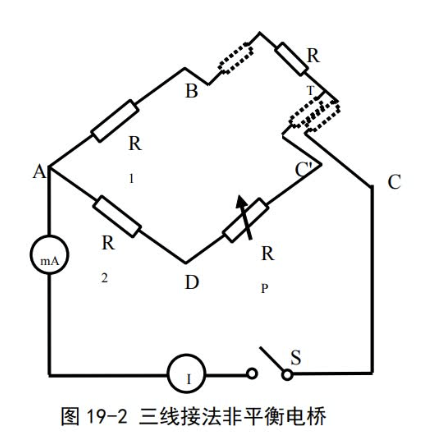
\includegraphics[height=7.3cm,width=7.5cm]{p2.png}
  
  \caption{fig1}
  \label{4}
  
  \end{figure}

\section{数据处理}

\noindent \textbf{实验条件:}E=19V,桥臂的实测值为$R_1=10.03k\Omega$,$R_2=9.98k\Omega$

\begin{center}
  \begin{tabular}{|c|c|c|c|c|c|c|c|}
    \hline
    T/°C&0.20&20.10 & 36.01 & 49.02&68.50&83.01&100.11\\
    \hline
    $U_{out}(mV)$ &0.05&13.89&25.04&34.01&47.70&58.04&69.84\\
    \hline
    
    

  \end{tabular}
  \begin{figure}[ht]
    \centering 
    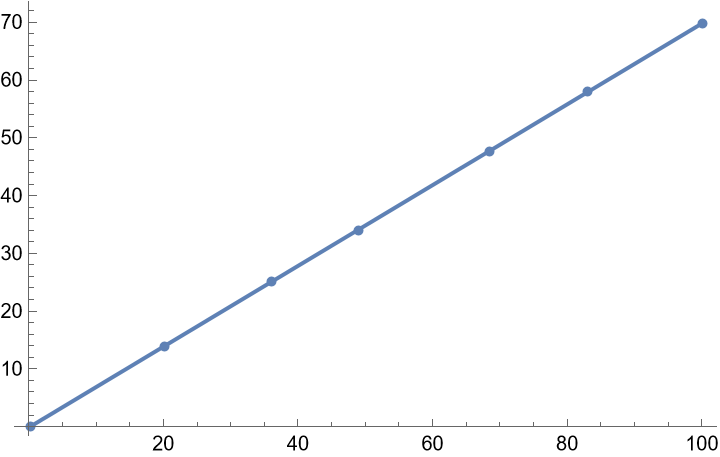
\includegraphics[height=6.0cm,width=7.5cm]{p3.png}
    
    \caption{fig2}
    \label{4}
    
    \end{figure}
  
\end{center}

\noindent 计算得到
$$A=\frac{2k}{I_0R_0}=3.784\times 10^{-3}°C^{-1}$$
计算A的不确定度
$$\sigma_k=k\times \sqrt{\frac{1/r^2-1}{n-2}}=0.090mV/°C$$
$$\sigma_{I_0}=e/\sqrt{3}=0.01mA$$
$$\sigma_{R_0}=e/\sqrt{3}=0.06\Omega$$
$$\sigma_A=A\sqrt{(\frac{2\sigma_k}{I_0R_0})^2+(\frac{2\sigma_{I_0}k}{I_0^2R_0})^2+(\frac{2\sigma_{R_0}k}{I_0R_0^2})^2}=2\times 10^{-6}°C^{-1}$$

\noindent 得到最终测量结果为:
$$A=(3.784\pm0.002)\times 10^{-3}°C^{-1}$$

\section{分析与讨论}
\noindent \textbf{实验中未考虑的误差:}本次实验中可能存在一些未被计算在内的误差,笔者认为主要是以下几点:

\noindent i.公式本身是线性近似的公式,可能存在高阶项导致的误差

\noindent ii.多用表不是理想电压表,电压表阻值不是无穷大导致的电压-温度相对完全线性存在一定偏离

\noindent iii.温度的测量和读数误差未被考虑在内

\noindent iv.仪器可能存在未定的系统误差,在处理数据时未作详细考虑


\end{document}